\documentclass[12pt]{article}

% Packages
\usepackage[margin=1in]{geometry}
\usepackage{setspace}
\usepackage{amsmath}
\usepackage{amssymb}
\usepackage{graphicx}
\usepackage{xcolor}
\usepackage{booktabs}
\usepackage{array}
\usepackage{tabularx}
\usepackage{hyperref}

% Title information
\title{Optimal Flood Policy}
\author{Taco Prins, Lennard Schlattmann, and Daniel Jonas Schmidt}
\date{\today}

\begin{document}

\maketitle

\section{Motivation}
\begin{itemize}
    \item Households have heterogeneous flood risk beliefs. Those who underestimate flood risk may not buy insurance or invest enough in private adaptation measures. A universal flood insurance mandate, which would ensure that even those who underestimate flood risk are insured, is often legally and politically infeasible.
    \item This creates a potential role for government intervention in the form of flood insurance subsidies, subsidies for private adaptation measures, disaster relief programs, or a combination of all policies.
    \item Subsidies can increase insurance and adaptation towards their socially optimal level, but with sufficient heterogeneity in beliefs, there will always be a group of households that underestimate flood risk enough to stay uninsured and under-adapted even with subsidies in place. 
    \item Disaster relief programs provide a safety net for uninsured households, but they also reduce incentives to buy flood insurance or invest in private adaptation measures. 
    \item What is the socially optimal mix of these policies in the presence of heterogeneous flood risk beliefs? Is it optimal to use all available policy instruments, or only a subset? How close is the current US policy to the optimum?
\end{itemize}

\section{Baseline model}

Consider a one-period model with one region. The government has a fixed budget $B$ dedicated to flood policies and can choose between two instruments: an insurance subsidy $s$ and a disaster relief fraction $a$.

\subsection{Household Problem}

Each household has wealth $w$ and faces a flood that occurs with true probability $p$ and causes damage $d$. Households differ in their subjective flood probability $q$, distributed across the population according to the CDF $F(q)$. There is no misperception about damage conditional on flood occurrence.

\begin{itemize}
    \item The government subsidizes flood insurance relative to the actuarially fair price, so an insured household pays $(1-s)pd$.
    \item The government provides disaster relief covering a fraction $a$ of damage for uninsured households that experience a flood.
\end{itemize}

\subsubsection*{Value Functions}

From the perspective of the social planner, the value functions for insured and uninsured households are given by
\begin{align}
    V_I(s) &= u(c_I) \\
    V_U(a) &= (1-p)\,u(c_{U,N}) + p\,u(c_{U,F}) = u(c_{U,N}) - p\cdot \Delta u
\end{align}
where 
\begin{itemize}
    \item $c_I = w - (1-s)pd$ is the consumption of an insured household,
    \item $c_{U,N} = w$ is that of an uninsured household that does not experience a flood,
    \item $c_{U,F} = w - (1-a)d$ is that of an uninsured household that experiences a flood, and
    \item $\Delta u \equiv u(c_{U,N}) - u(c_{U,F}) > 0$ is the utility loss from a flood for an uninsured household.
\end{itemize}
From the perspective of an uninsured household with subjective flood probability $q$, the expected utility is
\begin{align}
    \tilde{V}_U(q,a) = (1-q)\,u(c_{U,N}) + q\,u(c_{U,F}) = u(c_{U,N}) - q\cdot \Delta u
\end{align}

\subsubsection*{Optimal Behavior}
A household buys insurance if $V_I(s) > \tilde{V}_U(q,a)$. Setting $V_I(s) = \tilde{V}_U(q^*,a)$ yields
\begin{align}
    q^*\cdot\Delta u = u(c_{U,N}) - u(c_I) \label{eq:qstar}
\end{align}
For the marginal household with $q = q^*$, the utility cost of facing flood risk at subjective probability $q^*$ equals the utility cost of the insurance premium. 
Households with $q > q^*(s,a)$ buy insurance; those with $q \leq q^*(s,a)$ do not.

\subsection{Government Problem}

The government maximizes social welfare subject to its budget constraint. The social planner evaluates household welfare using the true flood probability $p$. Denoting the insurance take-up rate by $I(s,a) = 1 - F(q^*(s,a))$, the government's problem is
\begin{equation}
    S(s,a) = V_I(s)\cdot I(s,a) + V_U(a)\cdot\bigl(1-I(s,a)\bigr) \label{eq:welfare}
\end{equation}
subject to
\begin{equation}
    B = pd\bigl[s\,I(s,a) + a\,\bigl(1-I(s,a)\bigr)\bigr]. \label{eq:budget}
\end{equation}
The Lagrangian is
\[
    \mathcal{L}(s,a,\lambda) = S(s,a) + \lambda\!\left[B - pd\bigl(s\,I(s,a) + a\,\bigl(1-I(s,a)\bigr)\bigr)\right],
\]
where $\lambda$ is the shadow value of the budget constraint.

\subsubsection*{First-Order Conditions}

\begin{align}
    \frac{\partial\mathcal{L}}{\partial s} &=
        (V_I-V_U)\,\frac{\partial I}{\partial s}
        + \frac{\partial V_I}{\partial s}\cdot I
        - \lambda\,pd\!\left[
            I + (s-a)\,\frac{\partial I}{\partial s}
        \right] = 0 \label{eq:foc_s} \\[12pt]
    \frac{\partial\mathcal{L}}{\partial a} &=
        (V_I-V_U)\,\frac{\partial I}{\partial a}
        + \frac{\partial V_U}{\partial a}\cdot(1-I)
        - \lambda\,pd\!\left[
            (1-I) + (s-a)\,\frac{\partial I}{\partial a}
        \right] = 0 \label{eq:foc_a}
\end{align}

\subsubsection*{Marginal Value of Public Funds}

Rearranging each first-order condition so that the welfare gain per dollar of fiscal cost equals $\lambda$ gives the marginal value of public funds (MVPF) for each instrument:

\begin{align}
    \text{MVPF}_s &= \frac{
        \dfrac{\partial V_I}{\partial s}\cdot I
         +  (V_I-V_U)\,\dfrac{\partial I}{\partial s}
    }{
        pd\!\left[I + (s-a)\,\dfrac{\partial I}{\partial s}\right]
    } \label{eq:mvpf_s_vf} \\[14pt]
    \text{MVPF}_a &= \frac{
        \dfrac{\partial V_U}{\partial a}\cdot(1-I)
         + (V_I-V_U)\,\dfrac{\partial I}{\partial a}
    }{
        pd\!\left[(1-I) + (s-a)\,\dfrac{\partial I}{\partial a}\right]
    } \label{eq:mvpf_a_vf}
\end{align}

\noindent The numerators capture the marginal welfare gain:
\begin{itemize}
    \item \textbf{Direct benefit to recipients.} The subsidy benefits all $I$ insured households by $\partial V_I/\partial s = pd\,u'(c_I)$ per unit; relief benefits all $1-I$ uninsured flood victims by $\partial V_U/\partial a = pd\,u'(c_{U,F})$ per unit. Because uninsured flood victims are poorer, their marginal utility is higher.
    \item \textbf{Internality correction.} Each instrument shifts households across the margin, generating a welfare change of $(V_I - V_U)$ per switcher. Since $V_I = \tilde{V}_U(q^*,a)$ at the margin, the welfare gap is
    \begin{equation}
        V_I - V_U = \tilde{V}_U(q^*,a) - V_U(a) = (p-q^*)\,\Delta u. \label{eq:internality}
    \end{equation}
    Following Allcott, Lockwood, and Taubinsky (2019), we call this the \emph{internality correction}. It is positive for the subsidy (underinsured households switch to coverage) and negative for relief (households crowd out of insurance).
\end{itemize}
The denominators capture the marginal fiscal cost:
\begin{itemize}
    \item \textbf{Direct cost.} The marginal cost is $pd$ per recipient: $pd\cdot I$ for the subsidy and $pd\cdot(1-I)$ for relief.
    \item \textbf{Fiscal externality.} A switcher moves from costing $apd$ to $spd$ (or vice versa), changing fiscal cost by $(s-a)pd$ per switcher.
    \item \textbf{Optimum.} At an interior optimum, $\mathrm{MVPF}_s = \mathrm{MVPF}_a = \lambda$: neither instrument can be improved at the margin. Away from the optimum, the marginal dollar should go to the instrument with the higher MVPF.
\end{itemize}

\subsubsection*{Take-up responses} 

Since insurance coverage $I = 1 - F(q^*)$ depends on the threshold belief $q^*$, the take-up responses $\partial I/\partial s$ and $\partial I/\partial a$ depend on how $q^*$ changes with each instrument:
\begin{align}
    \frac{\partial I}{\partial s} &= -f(q^*)\,\frac{\partial q^*}{\partial s}
    = \frac{f(q^*)\,pd\,u'(c_I)}{\Delta u}, \label{eq:dI_s} \\
    \frac{\partial I}{\partial a} &= -f(q^*)\,\frac{\partial q^*}{\partial a}
    = -\frac{f(q^*)\,q^*d\,u'(c_{U,F})}{\Delta u}. \label{eq:dI_a}
\end{align}
\begin{itemize}
    \item \textbf{Density at the margin.} $f(q^*)$ amplifies both responses equally: a denser margin means more near-indifferent households react to any shift in $q^*$.

    \item \textbf{Sensitivity of $q^*$ to the subsidy.}
    Differentiate the indifference condition~\eqref{eq:qstar}, $q^*\cdot\Delta u = u(c_{U,N})-u(c_I)$, with respect to $s$. The right-hand side falls by $pd\,u'(c_I)$ — the unit subsidy lowers the premium by $pd$, reducing its utility cost by $pd\,u'(c_I)$. The left-hand side changes as $\frac{\partial q^*}{\partial s}\cdot\Delta u$, since $\Delta u$ is unaffected by $s$. Setting these equal gives $\frac{\partial q^*}{\partial s}=-\frac{pd\,u'(c_I)}{\Delta u}$. The denominator $\Delta u$ is the exchange rate from probability units to utility in the indifference condition: one unit of $q^*$ costs $\Delta u$ in expected flood-risk utility, so dividing by $\Delta u$ converts a utility saving back into a probability-threshold shift. Higher flood stakes ($\Delta u$ large) mean each unit of belief is already expensive, so the same premium cut achieves a smaller threshold reduction.

    \item \textbf{Sensitivity of $q^*$ to relief.}
    Differentiate the same condition with respect to $a$. The right-hand side is unchanged — relief does not affect the insurance premium. The left-hand side changes via the product rule: $\frac{\partial q^*}{\partial a}\cdot\Delta u + q^*\cdot\frac{\partial\Delta u}{\partial a}=0$. A unit increase in $a$ raises $c_{U,F}$ by $d$, so $\Delta u$ falls by $u'(c_{U,F})\cdot d$. Solving gives $\frac{\partial q^*}{\partial a} = \frac{q^*\cdot u'(c_{U,F})\cdot d}{\Delta u}$. The $q^*$ in the numerator comes directly from the product rule: it is the weight the marginal household already places on flood outcomes in the indifference condition, so the first-order impact of a reduction in $\Delta u$ on the left-hand side is proportional to $q^*$ itself. A household barely perceiving flood risk ($q^*\approx 0$) is almost unmoved by better relief; a household with correct beliefs ($q^*=p$) would crowd out at rate $pd$. Since $q^*<p$, crowd-out is always weaker than the crowd-in induced by an equal-cost subsidy.
\end{itemize}

\subsubsection*{MVPF in terms of deep parameters}

The deep-parameter formulas are obtained in two steps. First, substitute $\partial V_I/\partial s=pd\,u'(c_I)$, $\partial V_U/\partial a=pd\,u'(c_{U,F})$, $V_I-V_U=(p-q^*)\Delta u$, and the take-up responses~\eqref{eq:dI_s}--\eqref{eq:dI_a} into~\eqref{eq:mvpf_s_vf}--\eqref{eq:mvpf_a_vf}. Second, cancel the common factor $pd$ between numerator and denominator:
\begin{align}
    \text{MVPF}_s &= \frac{u'(c_I)\bigl[I + (p-q^*)\,f(q^*)\bigr]}{I + (s-a)\,\dfrac{pd\,u'(c_I)\,f(q^*)}{\Delta u}}, \label{eq:mvpf_s} \\[14pt]
    \text{MVPF}_a &= \frac{u'(c_{U,F})\!\left[(1-I) - \dfrac{(p-q^*)q^*f(q^*)}{p}\right]}{(1-I) - (s-a)\,\dfrac{q^*d\,u'(c_{U,F})\,f(q^*)}{\Delta u}}. \label{eq:mvpf_a}
\end{align}

\begin{itemize}
    \item \textbf{$\Delta u$ cancels in the internality term.} The internality term in $\mathrm{MVPF}_s$ is $(p-q^*)\Delta u\cdot\frac{f(q^*)pd\,u'(c_I)}{\Delta u}$: the $\Delta u$ in the welfare gap and the $1/\Delta u$ in the take-up response cancel, since the welfare gain per switcher grows with flood stakes at exactly the rate the threshold becomes harder to shift. The remaining $pd\,u'(c_I)$ cancels with the $pd$ in the denominator, leaving $(p-q^*)f(q^*)u'(c_I)$. The same applies in $\mathrm{MVPF}_a$, leaving $-(p-q^*)\frac{q^*}{p}f(q^*)u'(c_{U,F})$.

    \item \textbf{Marginal utility times effective recipient count.} Each numerator factors as $u'(c_j)\times[\text{effective recipient count}]$. The inframarginal share ($I$ or $1-I$) is the direct contribution. The internality adds a belief-gap correction: each marginal household contributes its probability mistake $(p-q^*)$ to the effective count, since after the $\Delta u$ cancellation the welfare gain per switcher in $u'$-normalized units is simply $(p-q^*)$.

    \item \textbf{The $q^*/p$ discount in $\mathrm{MVPF}_a$.} The crowd-out correction is smaller by $q^*/p<1$, inheriting from the weaker behavioral response to relief ($q^*d$ vs.\ $pd$). The internality $(p-q^*)$ is the same for both instruments; the asymmetry comes entirely from the take-up response.

    \item \textbf{Limiting case.} When $f(q^*)=0$, all behavioral terms vanish: $\mathrm{MVPF}_s=u'(c_I)$ and $\mathrm{MVPF}_a=u'(c_{U,F})$. 
\end{itemize}

\subsection{Calibration}

TODO: fill table, double-check Lennard's numbers, find different sources for elasticity

\begin{table}[h!]
\centering
\caption{Calibration parameters}
\label{tab:calibration}
\begin{tabular}{llcc}
\toprule
Name & Symbol & Value & Source \\
\midrule \midrule
CRRA coefficient & $\gamma$ & 2 & Standard value\\
\midrule
Household wealth (normalized) & $w$ & 1 & \\
Average flood damage (share of home value) & $d$ & 0.15 & NFIP claims \\
Annual flood probability & $p$ & 0.01 & SFHA definition \\
\midrule
Insurance subsidy & $s$ & 0.3 & \\
Disaster relief fraction & $a$ & 0.05 &  \\
\midrule
Insurance take-up rate & $I$ & 0.5 & \\
Elasticity of take-up w.r.t.\ premium & $\varepsilon$ & -1 & \\
\bottomrule
\end{tabular}
\end{table}

\paragraph{Preferences.}
We assume a CRRA utility function $u(c)=c^{1-\gamma}/(1-\gamma)$. We set $\gamma=2$, a standard benchmark in the macroeconomic and insurance literatures.

\paragraph{Flood risk.}
Wealth is normalized to $w=1$, so all monetary quantities are expressed as fractions of household wealth. The parameter $d$ captures average flood damage as a fraction of house value. We estimate this from National Flood Insurance Program (NFIP) claims data by computing average payouts relative to the insured value of the property.
We set the annual flood probability equal to the threshold that defines the Special Flood Hazard Area: $p=0.01$, corresponding to the 100-year floodplain. Properties inside the SFHA face an annual flood probability of at least 1\%.

\paragraph{Current policy.}

\paragraph{Belief distribution.}
No reliable data source directly measures the distribution of subjective flood risk beliefs. For an evaluation of the local optimality of the current policy, we only need the insurance coverage and the density at the margin, which we can recover from observed take-up responses to premium variation. For an evaluation of global counterfactual policies, we need the full belief distribution. We address this by fitting a parametric distribution to match the observed take-up rate and premium semi-elasticity.

\paragraph{Local evaluation: Recovering the belief density.}
Let $\pi=(1-s)pd$ denote the insurance premium. Define the elasticity of take-up with respect to the premium as
\[
    \varepsilon \equiv \frac{\pi}{I}\,\frac{\partial I}{\partial\pi} < 0.
\]
Differentiating the indifference condition $q^*\Delta u = u(w)-u(w-\pi)$ with respect to $\pi$ gives $\partial q^*/\partial\pi = u'(c_I)/\Delta u$. Since $I=1-F(q^*)$, it follows that
\[
    \frac{\partial I}{\partial\pi} = -\frac{f(q^*)\,u'(c_I)}{\Delta u}.
\]
Substituting $\partial I/\partial\pi = \varepsilon I/\pi$ and solving for $f(q^*)$:
\begin{equation}
    f(q^*) = -\varepsilon\,\frac{I}{\pi}\,\frac{\Delta u}{u'(c_I)}. \label{eq:fqstar}
\end{equation}
The elasticity $\varepsilon$ is the single empirical input: it can be estimated from variation in insurance premiums across households or over time. Given $\varepsilon$ and $I$, all remaining objects on the right-hand side---$\pi$, $\Delta u$, and $u'(c_I)$---are computable from the structural parameters $(w,d,s,a,\gamma)$.

\paragraph{Global evaluation: Fitting a parametric distribution.}
For global evaluations---tracing the optimal policy frontier or computing welfare at counterfactual policies far from the status quo---the complete distribution $F(q)$ is required. We fit a Beta distribution $q\sim\mathrm{Beta}(\alpha,\beta)$, whose two free parameters are identified by two moment conditions. Let $\hat{f} \equiv -\varepsilon(I/\pi)(\Delta u/u'(c_I))$ denote the target density derived in~\eqref{eq:fqstar}. The conditions are:
\begin{align}
    I_{q^*}(\alpha,\beta) &= 1 - I, \label{eq:beta_cdf} \\
    \frac{(q^*)^{\alpha-1}(1-q^*)^{\beta-1}}{B(\alpha,\beta)} &= \hat{f}, \label{eq:beta_pdf}
\end{align}
where $I_{q^*}(\alpha,\beta)$ is the regularized incomplete beta function and $B(\alpha,\beta)=\Gamma(\alpha)\Gamma(\beta)/\Gamma(\alpha+\beta)$. Condition~\eqref{eq:beta_cdf} requires the fraction of the population with beliefs at or below $q^*$ to equal the observed uninsured share $1-I$; condition~\eqref{eq:beta_pdf} requires the density at $q^*$ to equal the value pinned down by the premium elasticity. Given the structural objects $(q^*,\pi,\Delta u,u'(c_I))$---all computable from $(w,d,s,a,\gamma)$---together with the empirical inputs $(I,\varepsilon)$, the system~\eqref{eq:beta_cdf}--\eqref{eq:beta_pdf} uniquely identifies $(\alpha,\beta)$ and is solved numerically.

\subsection{Results}

TODO: add results

\section{Extensions}
\begin{itemize}
    \item Administration costs for flood insurance and disaster relief
    \item Private adaptation measures
    \item What is the optimal budget dedicated to flood policies? Compare marginal value of public funds with marginal cost of public funds
    \item Correlation of flood risk beliefs with income and/or wealth
    \item Heterogeneity in risk aversion
    \item Public adaptation measures
    \item Liquidity-provision policies (disaster loans, 401k withdrawals, mortgage relief)
    \item Households migrate into flood-prone areas because of government support (sorting based on beliefs)
    \item Continuous flood insurance decision
    \item Continuous flood damage
\end{itemize}

\subsection{Continuous flood damage}

Damage is now random: $\textcolor{red}{D\sim G}$ with mean $\textcolor{red}{\bar{d}\equiv\mathbb{E}[D]}$. All other primitives are unchanged.

\paragraph{Value functions.}
Insured consumption is $c_I=w-(1-s)p\textcolor{red}{\bar{d}}$. Uninsured flood consumption is realization-dependent: $c_{U,F}(\textcolor{red}{D})=w-(1-a)\textcolor{red}{D}$. The utility loss from a flood becomes
\[
    \textcolor{red}{\Delta u} \equiv u(c_{U,N}) - \textcolor{red}{\mathbb{E}[u(c_{U,F}(D))]},
\]
now a function of $a$. The value functions are
\begin{align}
    V_I(s) &= u(c_I), \\
    V_U(a) &= u(c_{U,N}) - p\cdot\textcolor{red}{\Delta u}, \\
    \tilde{V}_U(q,a) &= u(c_{U,N}) - q\cdot\textcolor{red}{\Delta u}.
\end{align}

\paragraph{Optimal behavior.}
The threshold condition is unchanged in form: $q^*\cdot\textcolor{red}{\Delta u}=u(c_{U,N})-u(c_I)$.

\paragraph{Government problem.}
Social welfare takes the same form~\eqref{eq:welfare}. The budget constraint replaces $d$ by $\textcolor{red}{\bar{d}}$:
\[
    B=p\textcolor{red}{\bar{d}}\bigl[s\,I(s,a)+a\,(1-I(s,a))\bigr].
\]

\paragraph{Marginal value of public funds.}
The internality correction retains the same form: $V_I-V_U=(p-q^*)\,\textcolor{red}{\Delta u}$. Writing $\textcolor{red}{\overline{Du'}\equiv\mathbb{E}[D\,u'(c_{U,F}(D))]}$, the direct marginal benefits and take-up responses are:
\begin{align}
    \frac{\partial V_I}{\partial s} &= p\textcolor{red}{\bar{d}}\,u'(c_I),
    &\frac{\partial I}{\partial s} &= \frac{f(q^*)\,p\textcolor{red}{\bar{d}}\,u'(c_I)}{\textcolor{red}{\Delta u}}, \label{eq:dI_s_cont}\\[6pt]
    \frac{\partial V_U}{\partial a} &= p\,\textcolor{red}{\overline{Du'}},
    &\frac{\partial I}{\partial a} &= -\frac{f(q^*)\,q^*\,\textcolor{red}{\overline{Du'}}}{\textcolor{red}{\Delta u}}. \label{eq:dI_a_cont}
\end{align}
The subsidy row is unchanged in form ($d\to\bar{d}$). For relief, $d\,u'(c_{U,F})$ is replaced by $\textcolor{red}{\overline{Du'}}$, which exceeds $\bar{d}\,u'(c_{U,F}(\bar{d}))$ under concavity. The $\Delta u$ cancellation and $p\bar{d}$ factorisation then proceed identically to the baseline:
\begin{align}
    \text{MVPF}_s &= \frac{u'(c_I)\bigl[I + (p-q^*)\,f(q^*)\bigr]}{I + (s-a)\,\dfrac{p\textcolor{red}{\bar{d}}\,u'(c_I)\,f(q^*)}{\textcolor{red}{\Delta u}}}, \label{eq:mvpf_s_cont}\\[14pt]
    \text{MVPF}_a &= \frac{\textcolor{red}{\dfrac{\overline{Du'}}{\bar{d}}}\!\left[(1-I) - \dfrac{(p-q^*)q^*f(q^*)}{p}\right]}{(1-I) - (s-a)\,\dfrac{q^*\,\textcolor{red}{\overline{Du'}}\,f(q^*)}{\textcolor{red}{\Delta u}}}. \label{eq:mvpf_a_cont}
\end{align}
$\mathrm{MVPF}_s$ is unchanged in form. In $\mathrm{MVPF}_a$, $u'(c_{U,F})$ is replaced by $\textcolor{red}{\overline{Du'}/\bar{d}}$.

\subsection{Risk aversion heterogeneity}

We now explicitly assume a CRRA utility function, i.e. $u(c)=\frac{c^{1-\gamma}}{1-\gamma}$. The marginal indifferent belief of an agent with CRRA $\gamma$ is 
\begin{equation}
    q^*(s,a;\gamma) = \frac{w^{1-\gamma} - (w-(1-s)pd)^{1-\gamma}}{w^{1-\gamma} - (w-(1-a)d)^{1-\gamma}}. \label{eq:qstargamma}
\end{equation}

Risk aversion $\gamma$ has a considerable affect on this threshold value. Figure \ref{fig:qstar_gamma} shows how $q^*$ varies with $\gamma$, using $s=13.9\%$ and $a=7.4\%$.
\begin{figure}[h!]
    \centering
    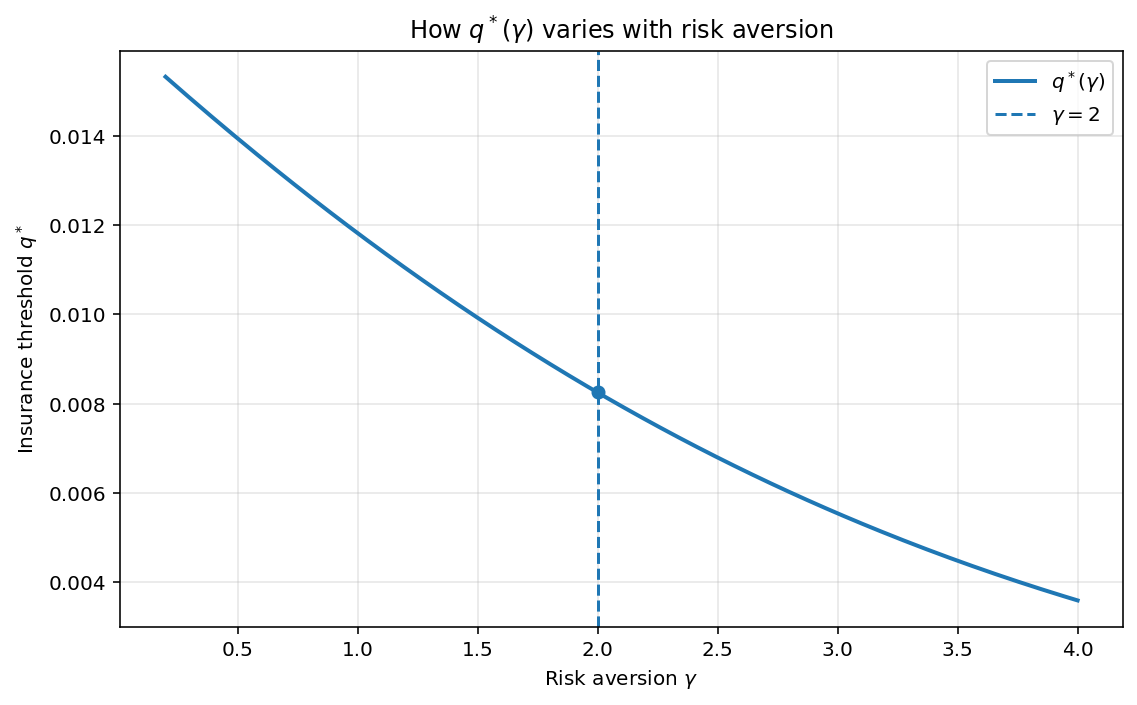
\includegraphics[width=0.7\linewidth]{figures/Dependence_q_gamma.png}
    \caption{Dependence of the insurance threshold $q^*$ on risk aversion $\gamma$, evaluated at $s=13.9\%$ and $a=7.4\%$.}
    \label{fig:qstar_gamma}
\end{figure}

However, dispersion in risk aversion does not seem to affect very much how the fraction of insured households responds to policy. Figure \ref{fig:fracinsuredgamma} below shows the fraction of insured households as a function of $a$, with $s$ adjusting to meet the government budget constraint. The left-hand panel shows this fraction with $\sigma=0.7\%$, and the right-hand panel with $\sigma=1.0\%$. CRRA $\gamma$ is assumed to follow a lognormal distribution with mean $2$. From this numerical evidence, dispersion in $\gamma$ thus does not alter by very much the fundamental trade-off between compensating flood-affected households and maximising insurance coverage.  
    
\begin{figure}[h]
\centering
\begin{minipage}{0.48\textwidth}
\centering
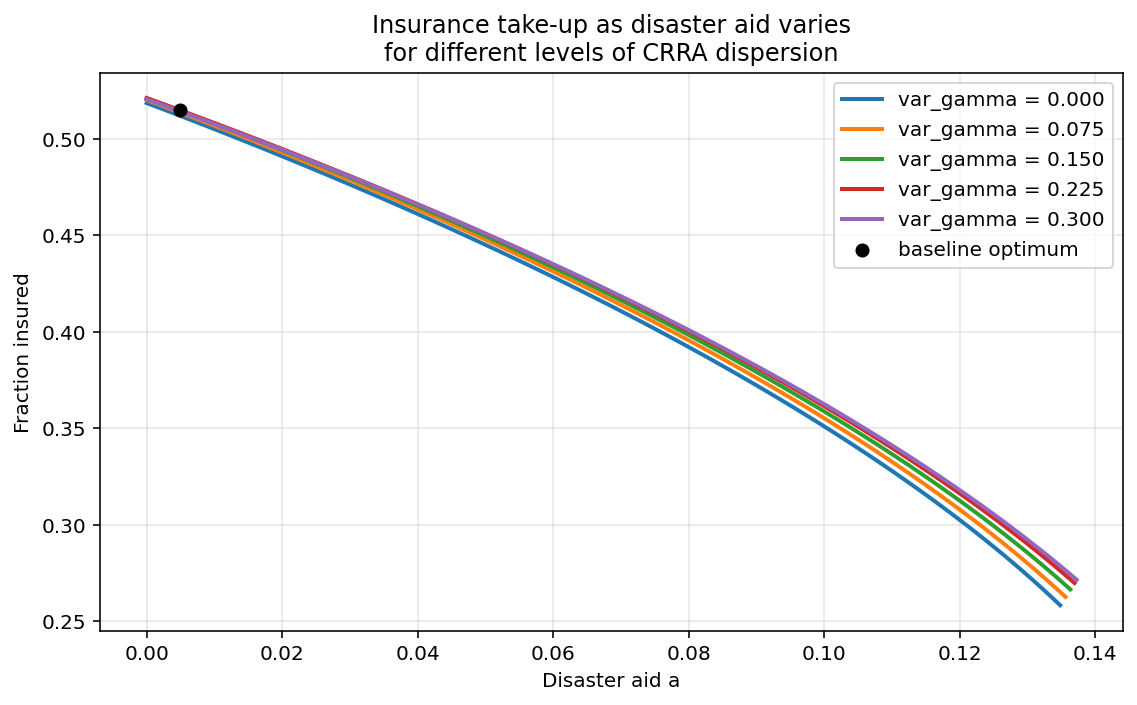
\includegraphics[width=\textwidth]{figures/Dependence_insuranceratio_vargamma.png}
\caption{Fraction of insured household as a function of policy $a,s$ and variance of CRRA $\gamma$, with $\sigma_q=0.7\%$}
\end{minipage}
\hfill
\begin{minipage}{0.48\textwidth}
\centering
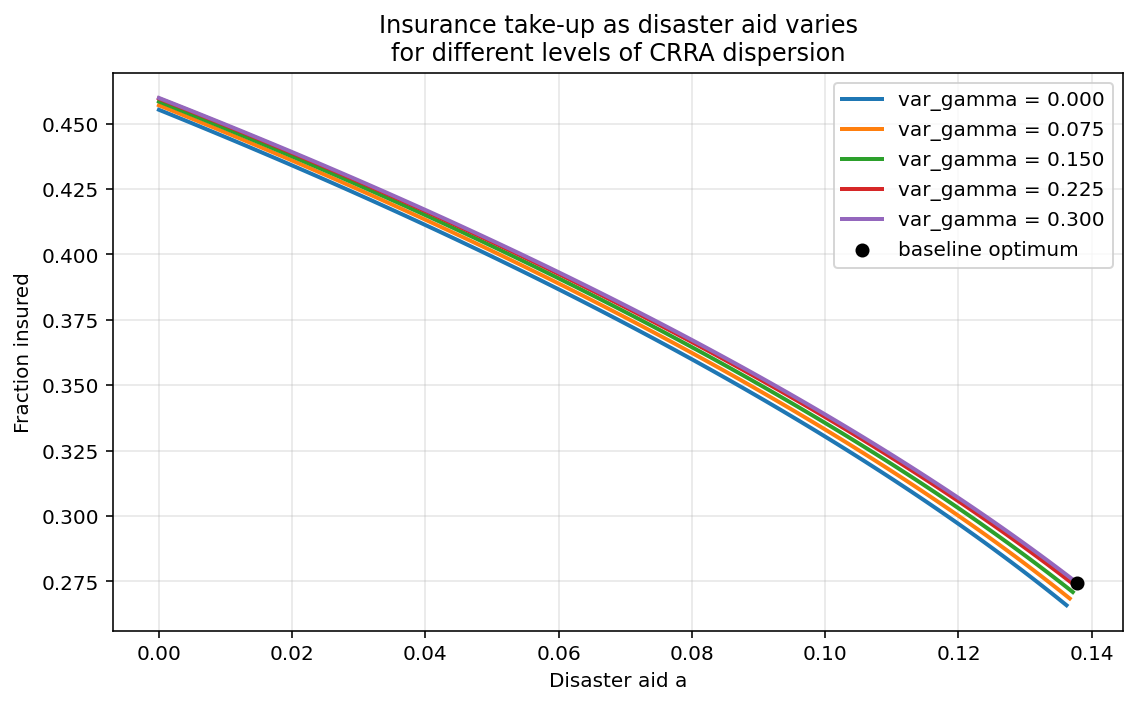
\includegraphics[width=\textwidth]{figures/Dependence_insuranceratio_vargamma_varq0.01.png}
\caption{Fraction of insured household as a function of policy $a,s$ and variance of CRRA $\gamma$, with $\sigma_q=1.0\%$}
\end{minipage}
\label{fig:fracinsuredgamma}
\end{figure}   

\subsubsection{Social planner problem with heterogeneous risk aversion}

We assume that risk aversion is heterogeneous across households, with
\[
\gamma \sim \text{LogNormal}(\mu_\gamma, \sigma_\gamma^2).
\]

When preferences are heterogeneous, utility is not directly comparable across individuals, as cardinal utility depends on the normalization of the utility function. To obtain a welfare measure that is comparable across households, we evaluate outcomes in terms of \emph{certainty-equivalent consumption}.

\paragraph{Certainty-equivalent consumption}

Fix a household with risk aversion $\gamma$. If the household purchases insurance, consumption is deterministic and given by
\[
c_I(s) = w - (1-s)\pi d.
\]
Hence, its certainty-equivalent consumption is simply
\[
c_I^{CE}(s;\gamma) = c_I(s).
\]

If instead the household remains uninsured, it faces flood risk. Expected utility is given by
\[
V_U(s,a;\gamma) = (1-p)u(w;\gamma) + p\,u\bigl(w-(1-a)d;\gamma\bigr),
\]
and the corresponding certainty-equivalent consumption $c_U^{CE}(s,a;\gamma)$ is implicitly defined by
\[
u\bigl(c_U^{CE}(s,a;\gamma);\gamma\bigr) = V_U(s,a;\gamma).
\]

\paragraph{Aggregation over belief heterogeneity}

Households differ in their subjective flood probability $q$, distributed according to a Beta distribution. For a given $\gamma$, households purchase insurance if and only if $q \geq q^*(s,a;\gamma)$, where $q^*(s,a;\gamma)$ is defined in \eqref{eq:qstargamma}. 

Let $F(\cdot)$ denote the CDF of the belief distribution. Then the fraction of households with risk aversion $\gamma$ that remains uninsured is $F\bigl(q^*(s,a;\gamma)\bigr)$, while the fraction that purchases insurance is $1 - F\bigl(q^*(s,a;\gamma)\bigr)$.

Average certainty-equivalent consumption for households with risk aversion $\gamma$ is therefore given by
\[
c^{CE}(s,a;\gamma)
=
F\bigl(q^*(s,a;\gamma)\bigr)\, c_U^{CE}(s,a;\gamma)
+
\bigl(1 - F\bigl(q^*(s,a;\gamma)\bigr)\bigr)\, c_I^{CE}(s;\gamma).
\]

\paragraph{Social welfare}

The social planner maximizes average certainty-equivalent consumption across the distribution of risk preferences:
\begin{equation}
S(s,a)
=
\int c^{CE}(s,a;\gamma)\, dG(\gamma),
\label{eq:welfarehetpreferences}
\end{equation}
where $G(\gamma)$ denotes the distribution of risk aversion.

\paragraph{Result}
When we implement this idea, we get the following result: preference heterogeneity pushes optimal policy away from disaster aid and towards the insurance subsidy. The intuition is probably that households that fail to insure on average have lower risk aversion. Hence, they lose less certainty-equivalent consumption from the realisation of flood losses. Since other things are approximately equal (the strength of the moral hazard effect from disaster aid does not really change, as we've seen), this pushes the social planner to value disaster aid less. Figure \ref{fig:optpolicy_gamma} illustrates the result, with $\sigma_q=0.7\%$. (The cases with $\sigma_q=0.5\%$ and $\sigma_q=1\%$ do not change.)

\begin{figure}[h!]
    \centering
    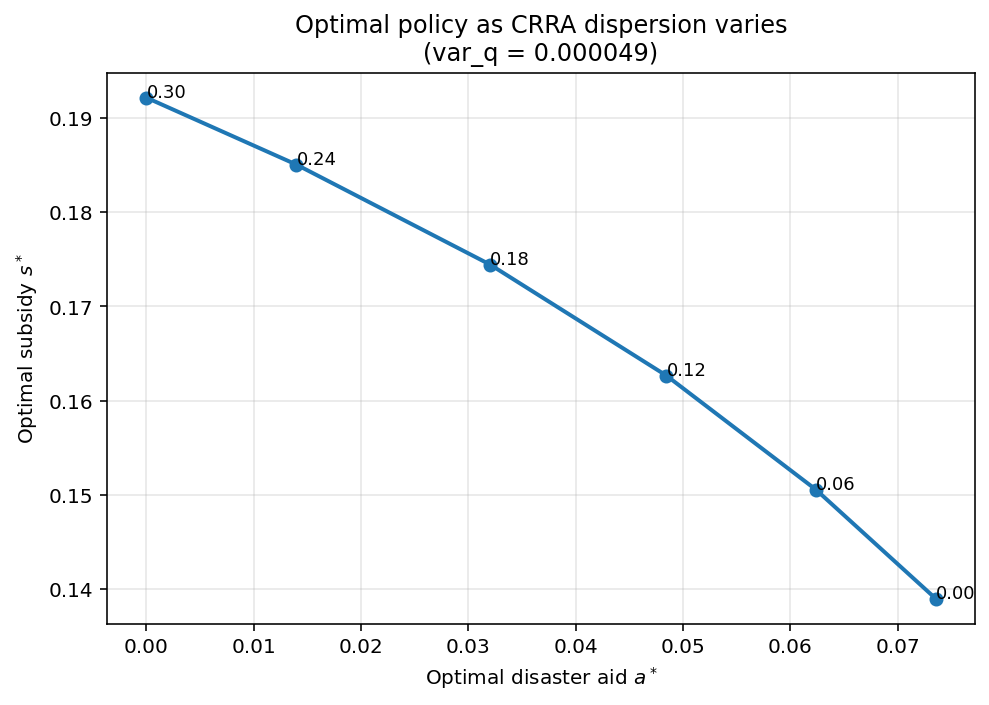
\includegraphics[width=0.7\linewidth]{figures/Dependence_optimalpolicy_vargamma.png}
    \caption{Optimal policy mix with $\sigma_q=0.7\%$. The dots indicate different levels of the variance of risk aversion $\gamma$.}
    \label{fig:optpolicy_gamma}
\end{figure}
\end{document}